\documentclass[11pt,a4paper,twoside]{book}
\usepackage[utf8]{inputenc}
\usepackage[spanish]{babel}
\usepackage{amsmath}
\usepackage{graphicx}
\usepackage{amsfonts}
\usepackage{amssymb}
\usepackage[left=2cm,right=2cm,top=2cm,bottom=2cm]{geometry}
\usepackage{float}
\author{Víctor de Tejada Molera}
\begin{document}
\chapter{Toma de datos}
	Para la realización de este proyecto, es necesaria la obtención de un gran número de respuestas al impulso en diferentes posiciones de una sala. En este capítulo, se repasan y analizan los criterios seguidos para la toma de los datos que posteriormente son procesados y utilizados en el test subjetivo de audio. Del mismo modo, se comenta el espacio escogido para la toma de los datos y el equipo utilizado.

	\section{Localización}

		\subsection{Descripción del espacio}

 			En nuestro caso particular, se ha optado por el salón de actos de la ETSIST ubicada en el Campus Sur de la UPM. Este salón de actos está diseñado como sala de conferencias y como espacio para actuaciones de música coral. 
 
 			El espacio tiene unas dimensiones de 25 metros de largo, por 13.64 metros de ancho. El auditorio tiene una altura aproximada de unos 5 metros aproximadamente.
 
 			El escenario se encuentra ligéramente levantado sobre el suelo del salón de actos mediante una estructura de madera. A los lados del escenario se encuentran unos paneles giratorios, también de madera, que dan acceso a dos bambalinas laterales. La parte trasera del escenario cuenta con un gran panel de madera situado en el centro de la pared. El techo del escenario cuenta con una concha acústica de madera y ocupa practicamente toda su superficie. El resto del techo se compone de paneles de madera ligeramente superpuestos y con ligera inclinación para evitar superficies paralelas.
 
 			Las paredes del auditorio se encuentran recubiertas en su mayoría por paneles de madera, excepto por una ligera zona acristalada hacia la zona superior. Las puertas situadas en los laterales son metálicas. 
 
 			La pared posterior, así como el resto de las paredes están compuestas principalmente de hydropanel y láminas de madera. En la parte trasera también se encuentra una pared metálica y una ventana acristalada que comunican con la sala de control.
 
 			El suelo de la zona más cercana al escenario está compuesto por láminas de madera, mientras que en la zona de butacas, se compone de linóleo.
 
 			Estos materiales pueden observarse en la figura \ref{fig:materiales}.
 
 			\begin{figure}
 				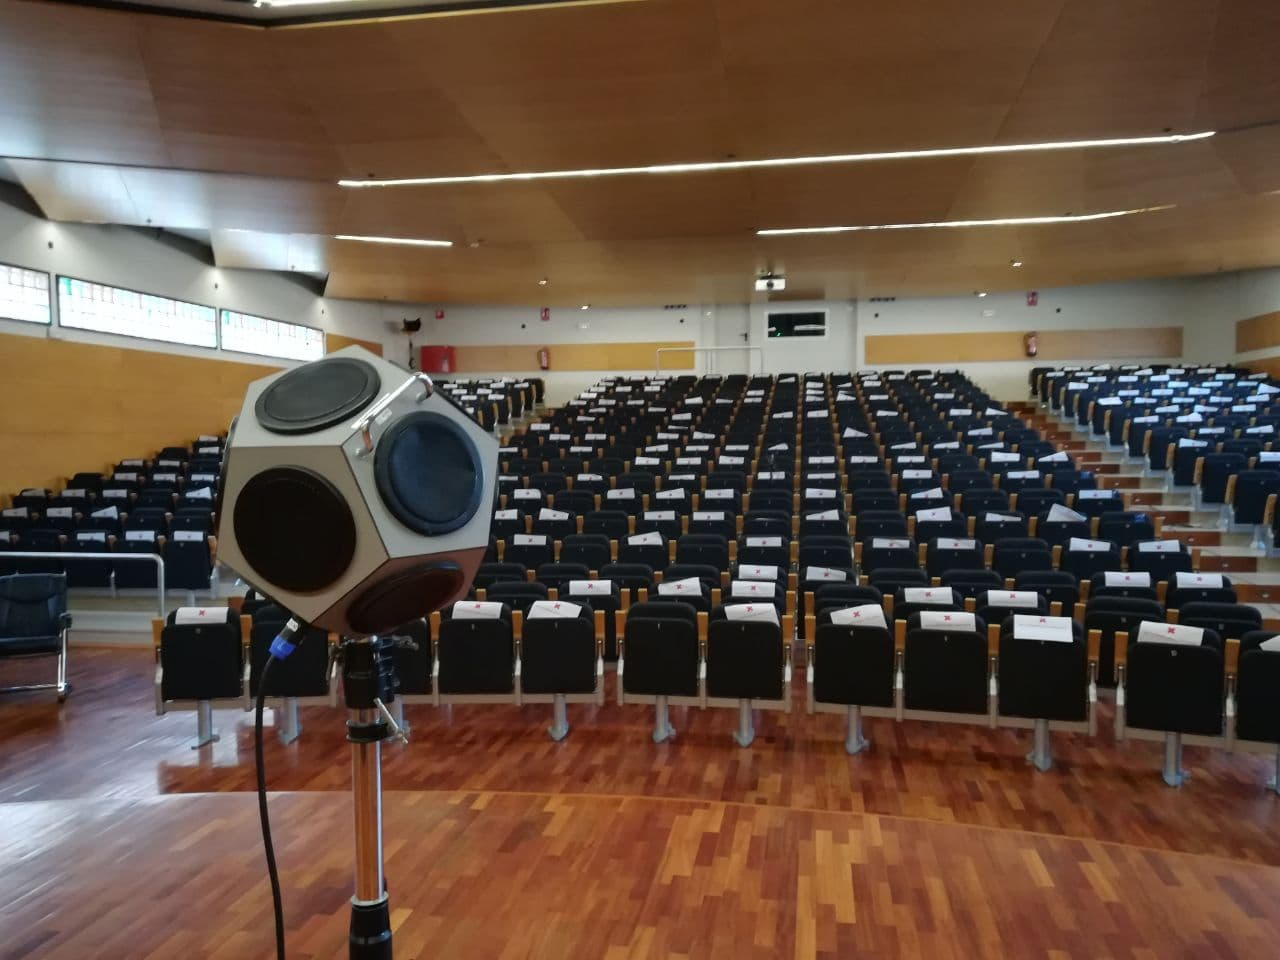
\includegraphics[scale=.25]{../imagenes/fuente.jpg}%
 				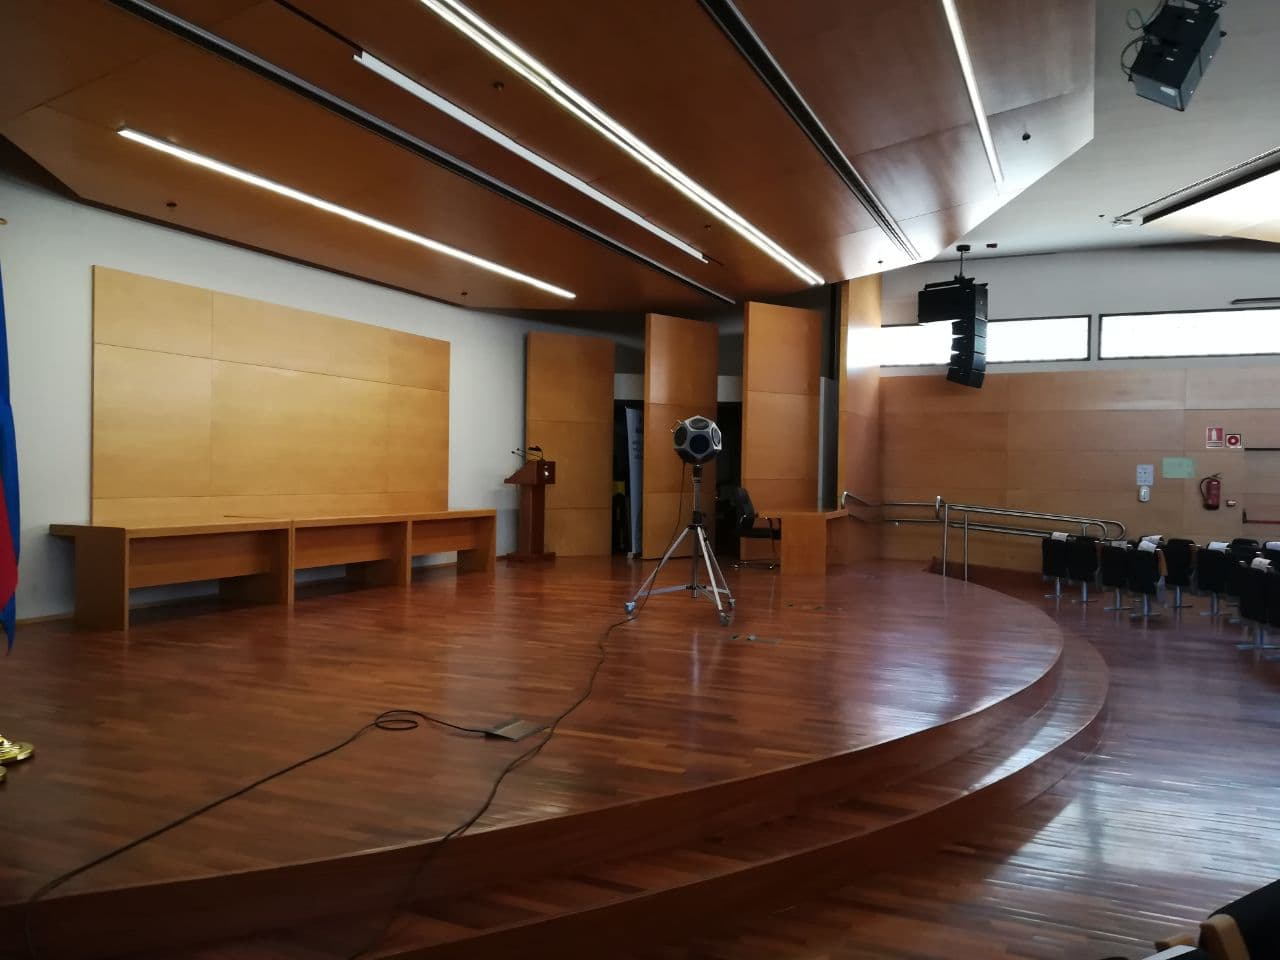
\includegraphics[scale=.25]{../imagenes/fuente2.jpg} 
 				\centering
 				\caption{El salón de actos de la ETSIST}
 				\label{fig:materiales}

 			\end{figure}
 


		\subsection{Distribución de las butacas}
			Este espacio está compuesto de dos zonas de butacas distintas:

 			Por un lado, dieciseis filas de butacas paralelas en escalera de veintiocho butacas cada una. Estas butacas se encuentran numeradas desde el centro hacia los extremos; los números pares se encuentran hacia la derecha (mirando hacia la zona de butacas) y los números impares se encuentran hacia la zona de la izquierda.
 
 			Por otro lado, existen otras dos filas de butacas situadas por delante del primer grupo. Estas tres filas se encuentran divididas, a su vez, en tres grupos: uno centrado y otro en cada lado (izquierda y derecha). La numeración sigue el mismo orden que las filas mostradas anteriormente. La numeración comienza en el centro del area central y los números pares se incrementan hacia la derecha. Esta numeración continúa en las zonas adyacentes como si se trataran de la misma fila. Se produce una situación análoga con las impares en la zona izquierda del auditorio.
 
 			En la figura \ref{fig:auditorio} se puede observar un esquema en planta del auditorio en el que se aprecian tanto las filas convencionales, como las areas adicionales.
			\begin{figure}
				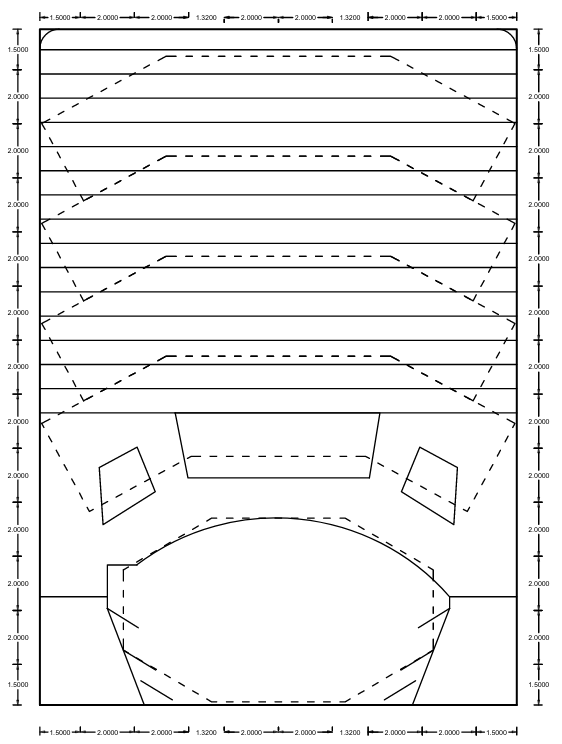
\includegraphics[scale=0.6]{../imagenes/auditorio.png}
				\centering
				\caption{Vista en planta del auditorio de la ETSIST}
				\label{fig:auditorio}
			\end{figure}
			
    \section{Primera toma de datos}
	    \subsection{Numeración y selección de las posiciones de toma de datos}
		    Como se plantea disponer de un gran número de respuestas al impulso, es importante determinar previamente un sistema para numerar inequívocamente las distintas posiciones en las que se van a tomar los datos. Por suerte, tanto las filas como las butacas ya se encuentran numeradas de antemano. Por ello, se decide mantener esta numeración para almacenar y referencias los datos de cada una de las posiciones. De esta forma, se tiene que para la zona de butacas paralelas la numeración es de la forma: ``FxBy''. Siendo ``x'' el número de la fila en la que se encuentra e ``y'' el número de la butaca.

		    Para la zona delantera, la numeración es ligéramente distinta y es de la forma ``AxBy''. Donde, de nuevo, ``x'' e ``y'' representan el número de fila y butaca respectivamente.

		    De esta forma, dos ejemplos pueden ser ``F3B27'' y ``A2B8''; siendo las posiciones de la butaca 27 de la fila 3 de butacas paralelas y la butaca 8 de la fila 3 de la zona delantera, respectivamente.

		    Con esta forma de numeración de butacas, se puede proceder a la selección de las diferentes posiciones en las que se obtienen las respuestas impulsivas de la sala. Para el caso de este proyecto, se ha supuesto que el salón de actos es simétrico en la parte izquierda y derecha. Por este motivo, se han determinado posiciones en la parte par de la sala. Después, se ha distribuido el área seleccionando una butaca y dejando butacas libres antes de seleccionar la siguiente posición para cada fila. Así mismo, para la fila siguiente no se selecciona la butaca que está en frente de la seleccionada, sino la inmediatamente a continuación a su derecha. De esta forma, se consigue un muestreo más uniforme de la sala. En la figura \ref{fig:butacasMarcadas} puede observarse un esquema con dicha distribución. 
		
		    \begin{figure}
	            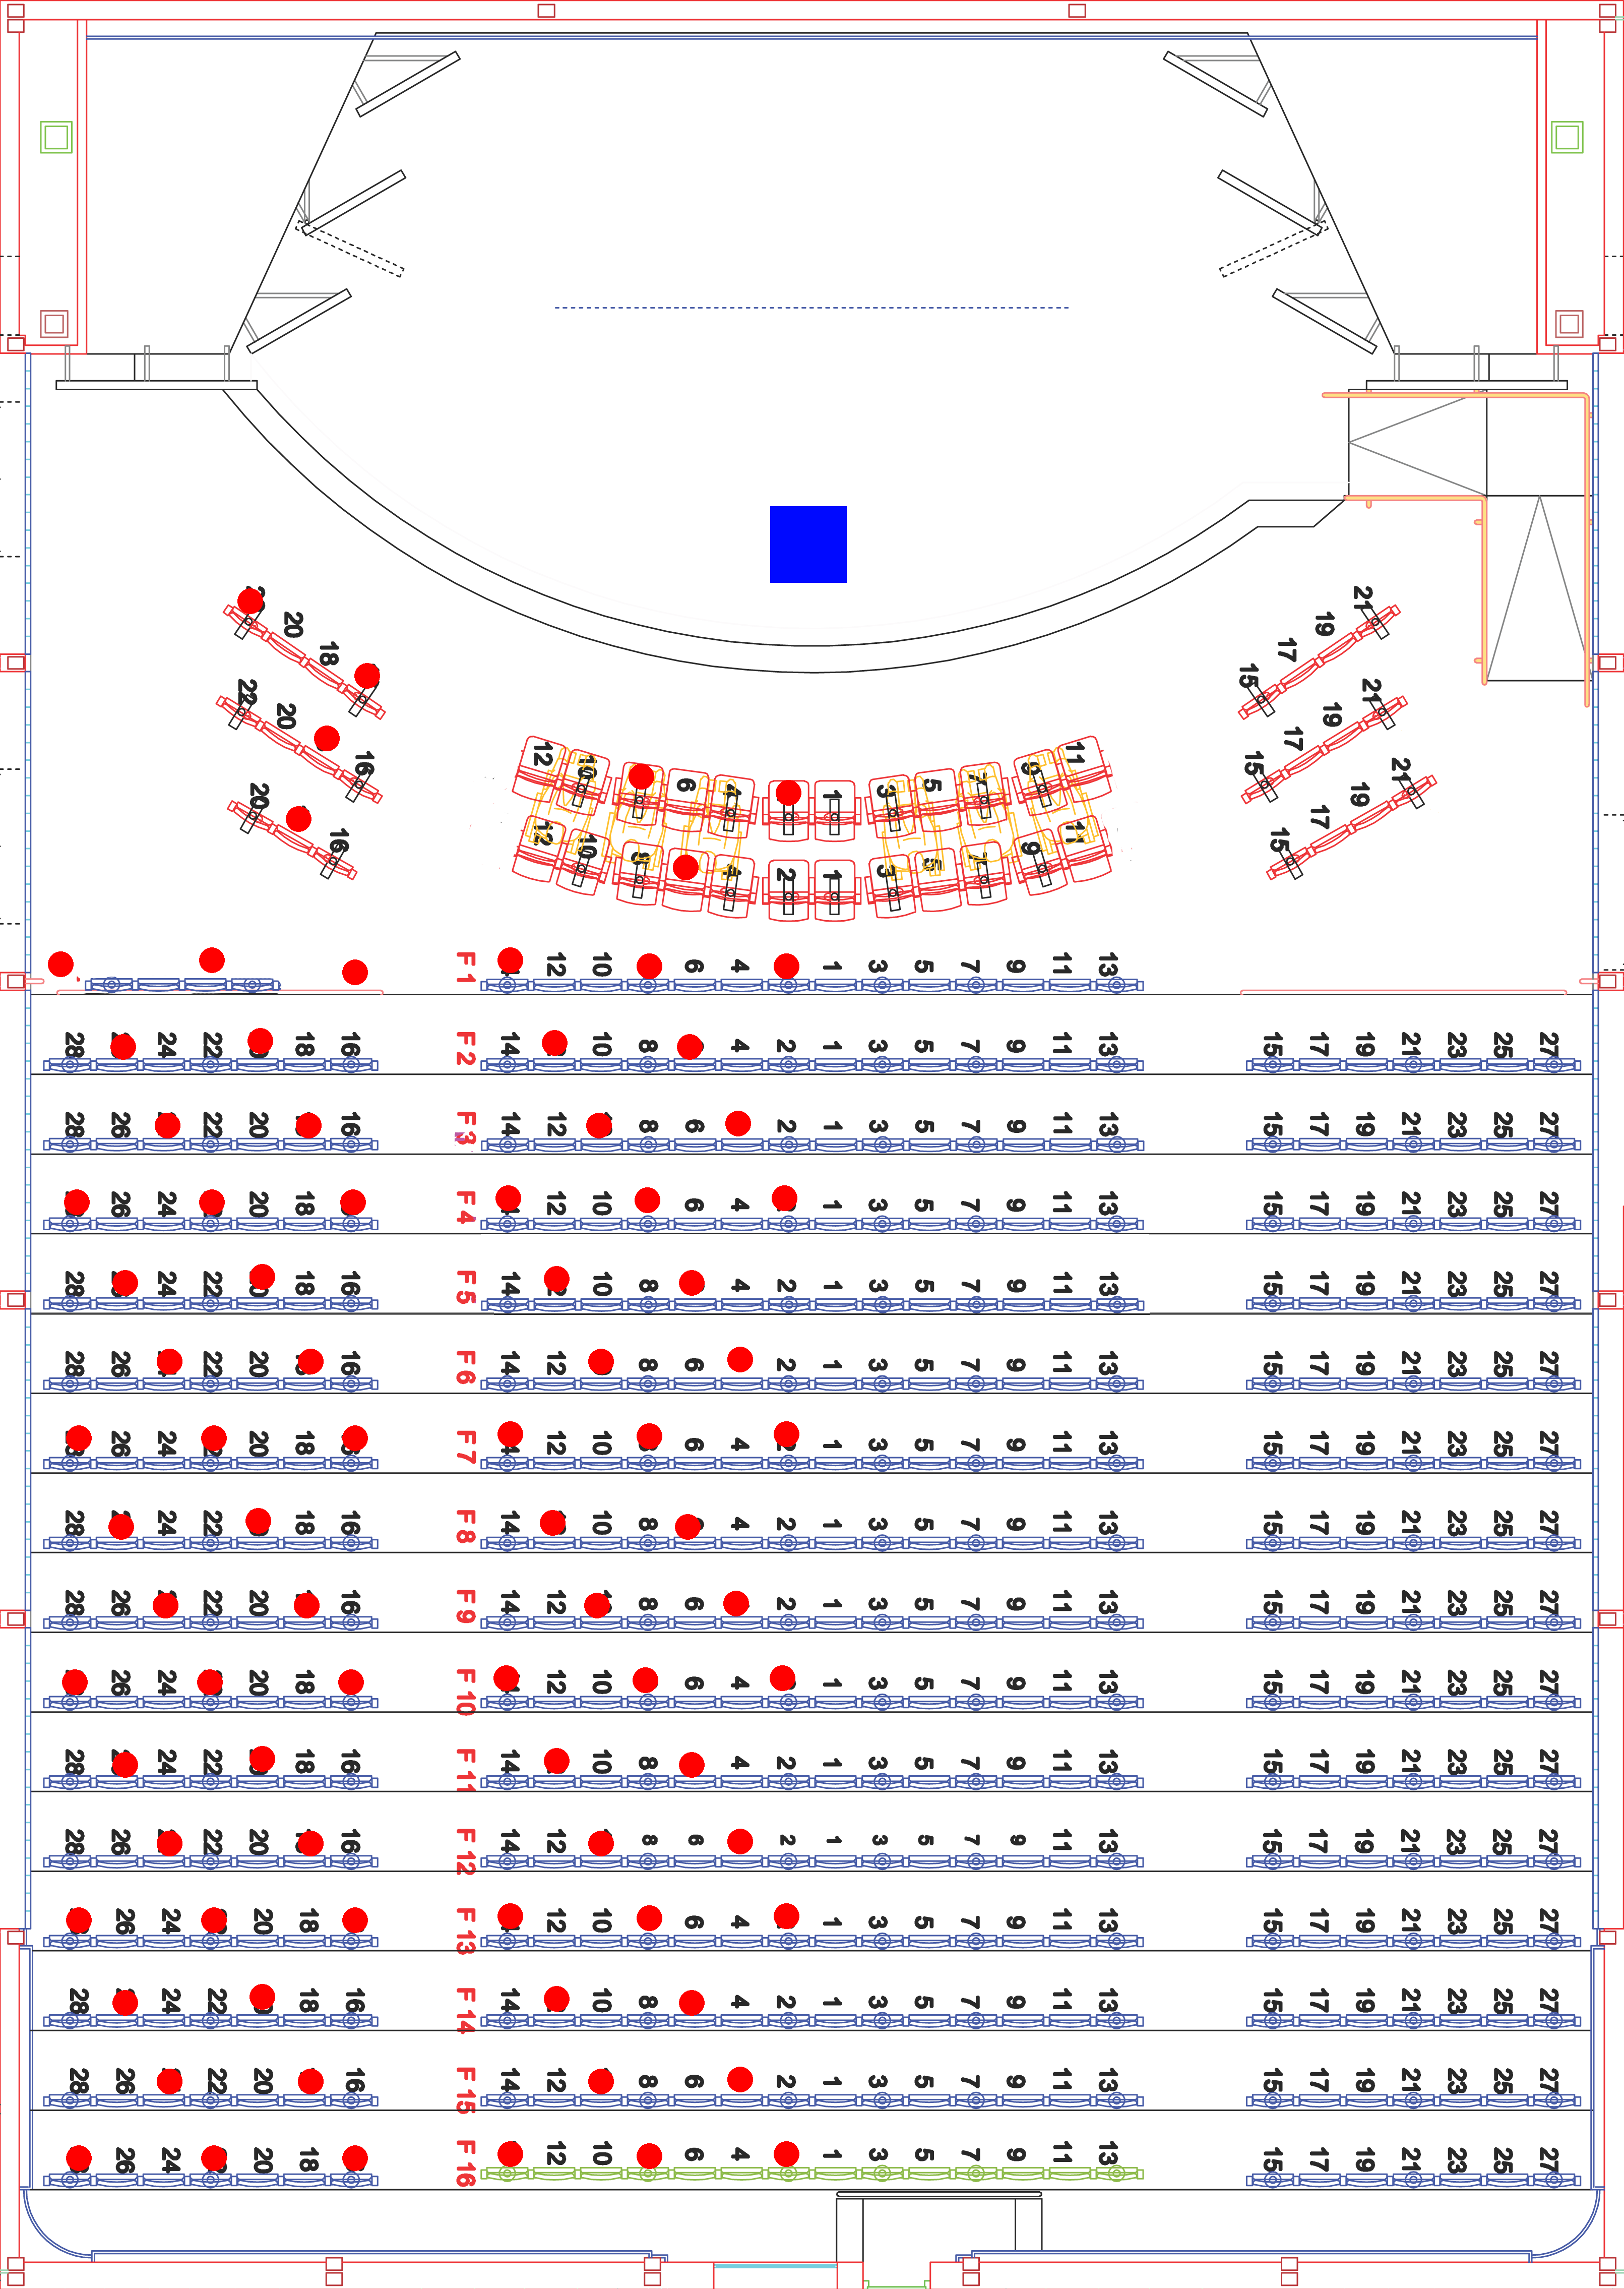
\includegraphics[scale=0.45]{../imagenes/auditorio_butacas_marcadas}
			    \centering
			    \caption{Distribución de las posiciones de grabación de las respuestas impulsivas. El cuadrado azul marca la posición de la fuente de sonido y los círculos rojos las posiciones de los micrófonos.}
			    \label{fig:butacasMarcadas}
	        \end{figure}

		    Como la toma de los datos se ha realizado en el transcurso de dos días, se ha optado por repetir las medidas en algunas posiciones. De esta forma se pretende obtener más información y asgurarnos de que la respuesta en dicha posición no varía en gran medida de un día para otro (por variaciones de temperatura, humedad, etc.). También se seleccionaron algunas posiciones de la parte impar del escenario. El motivo era para comprobar en la versión preliminar del test si nuestra hipótesis inical de la simetría de la sala era respaldada por las escuchas subjetivas de un pequeño número de participantes. Estas posiciones se encuentran en las posiciones extremas de la sala; es decir, las zonas más cercanas y lejanas al centro del escenario en la primera y última fila.

	    \subsection{Equipo utilizado para la toma de los datos}
	        Para la grabación de las respuestas impulsivas se ha utilizado el siguiente equipo:
	        \begin{itemize}
	            \item Ordenador portátil ASUS 2 con Windows 10 y software Dirac instalado.
	            \item Tarjeta de sonido MOTU UltraLite-mk3 Hybrid.
	            \item Amplificador de potencia Crown XLS 2002.
	            \item Fuente dodecaédrica.
	            \item Micrófono ominidireccional AKG-CK92.
	            \item Micrófono bidireccional AKG-CK94.
	            \item Alargaderas y cableado necesario para el conexionado de los equipos.
	            \item trípodes y sujecciones para los micrófonos.
	        
	        \end{itemize}
	    
	        En la figura \ref{fig:equipos} se pueden observar imágenes sobre varios de dichos equipos, y en la figura \ref{fig:control} se muestra cómo se organiza la zona de control para la realización de las medidas ubicada dentro del mismo salón de actos.
	    
	        \begin{figure}[H]
	            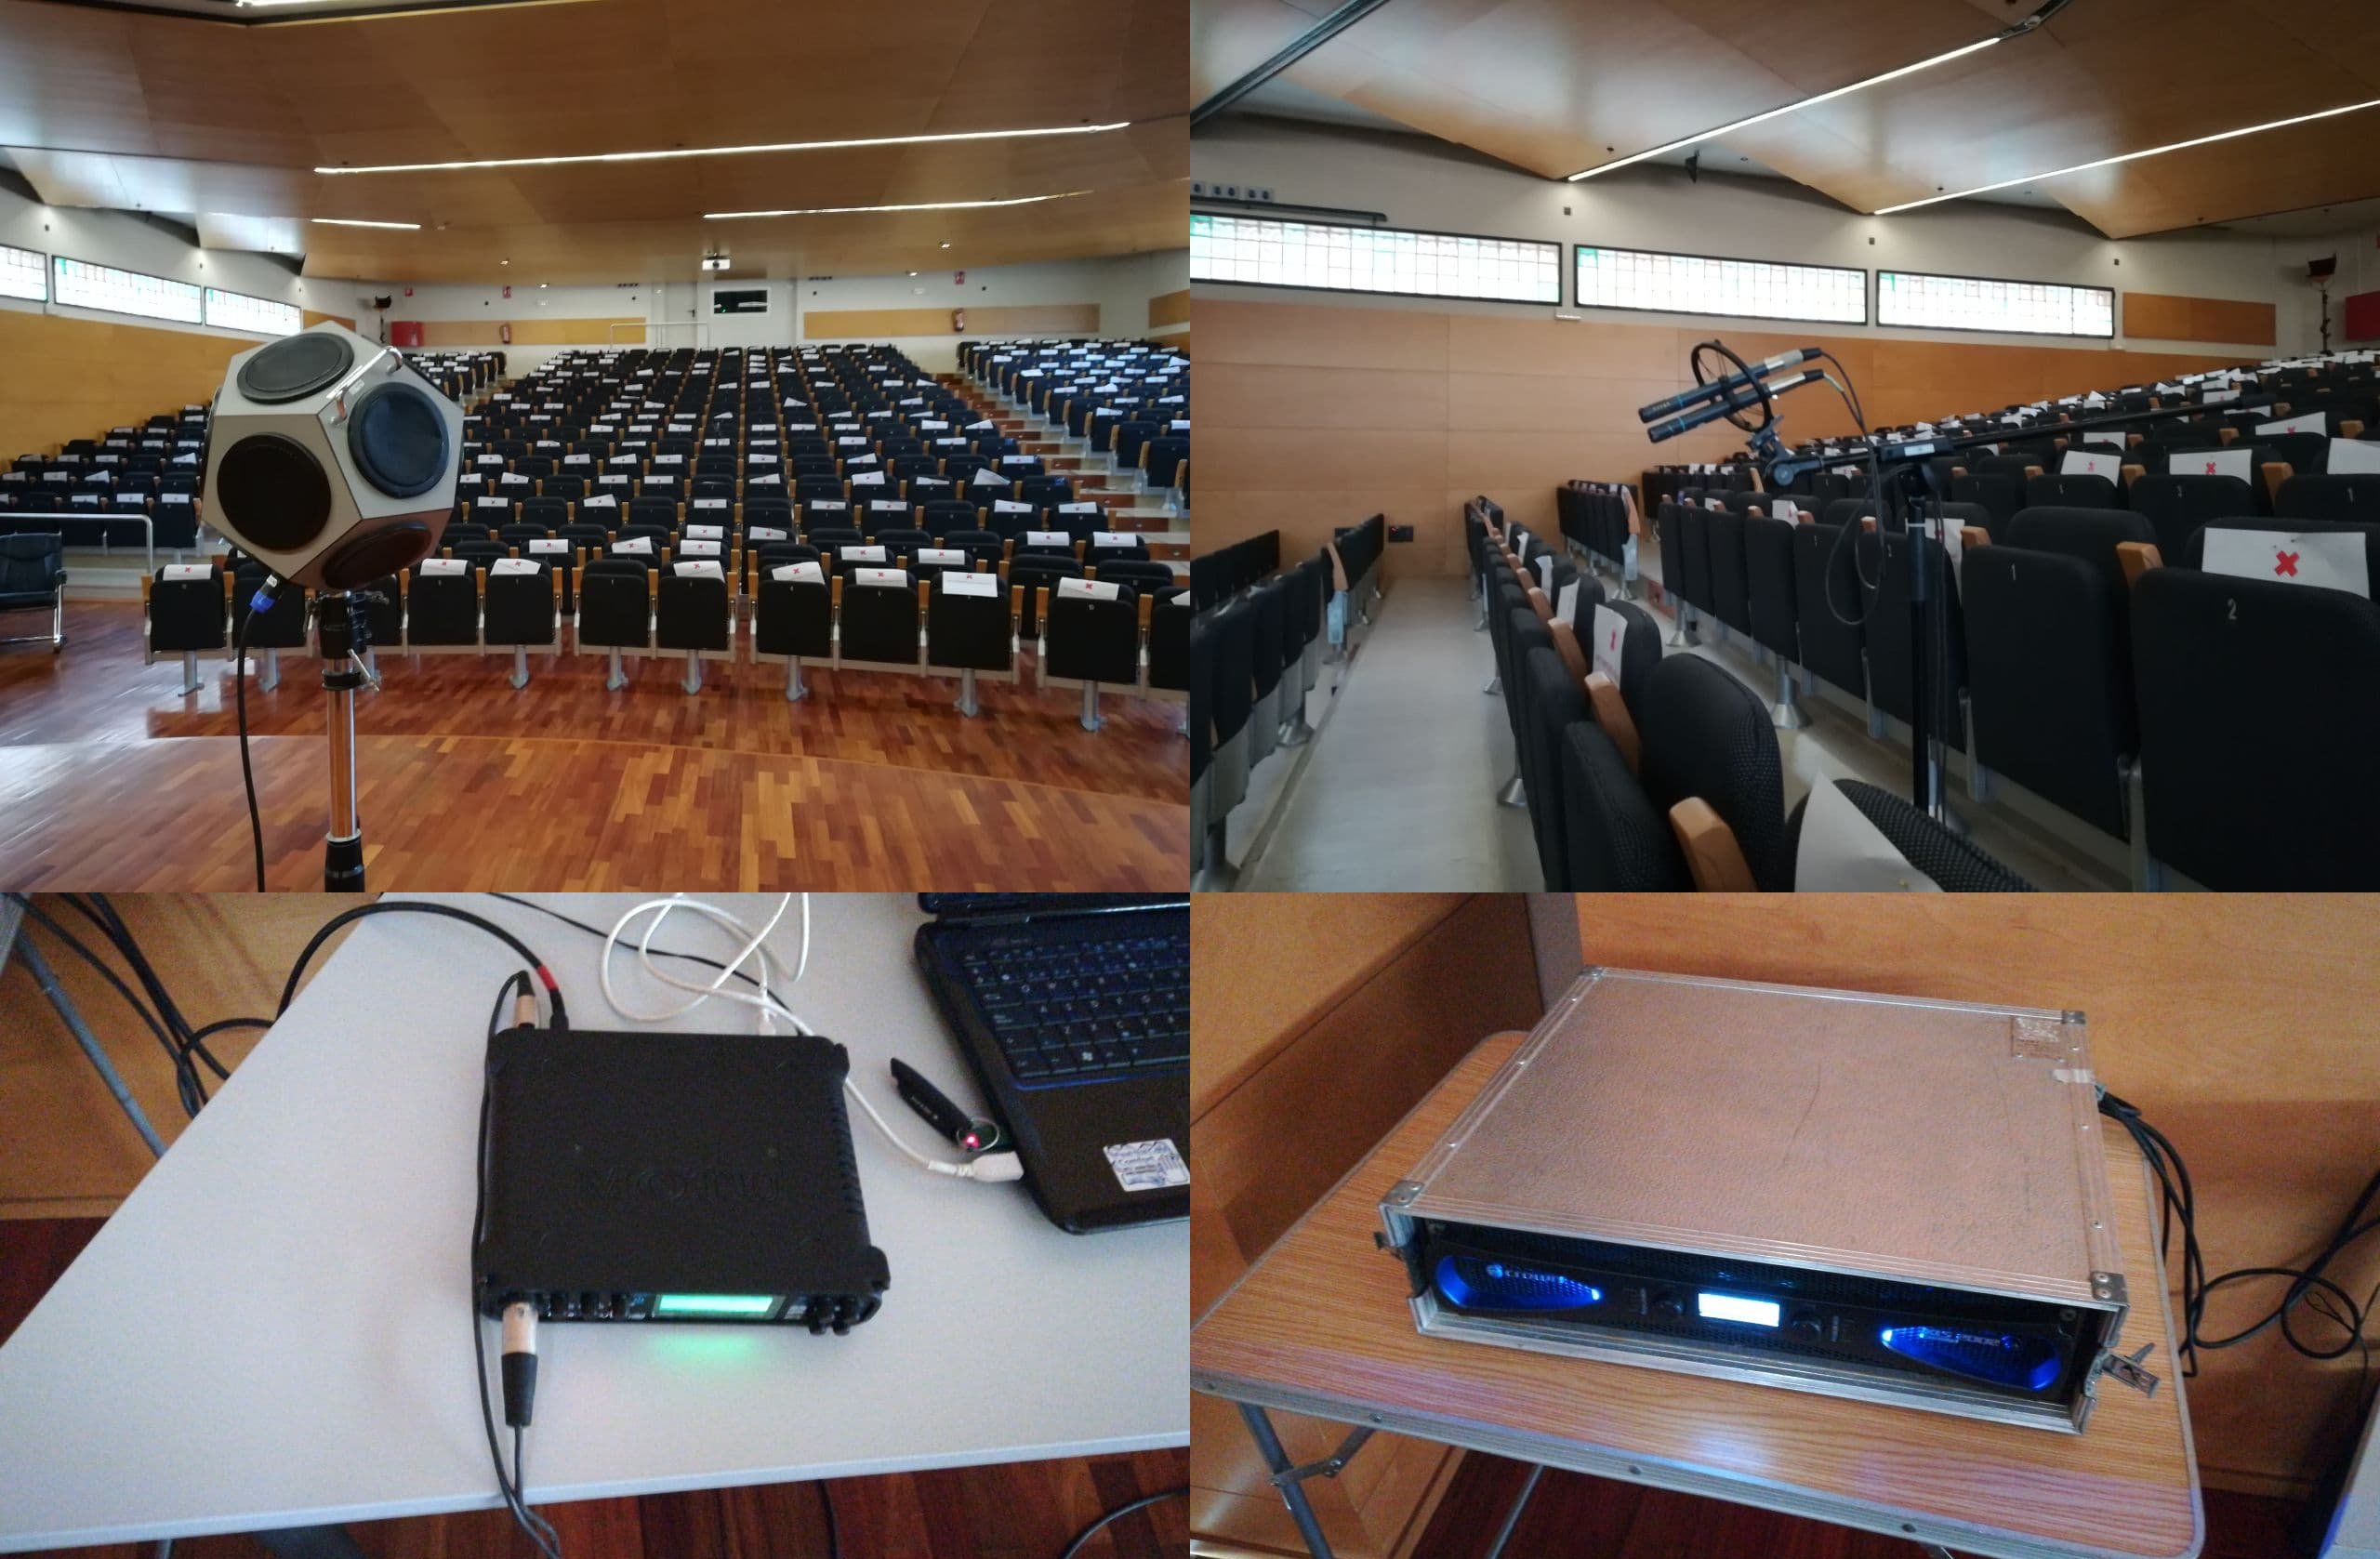
\includegraphics[scale=0.6]{../imagenes/equipos.jpg}
			    \centering
			    \caption{De izquierda a derecha y arriba a abajo: Fuente dodecaédrica, disposición de los micrófonos de medida, tarjeta de sonido MOTU y amplificador de potencia Crown.}
			    \label{fig:equipos}
	        \end{figure}
	    
	        \begin{figure}
	            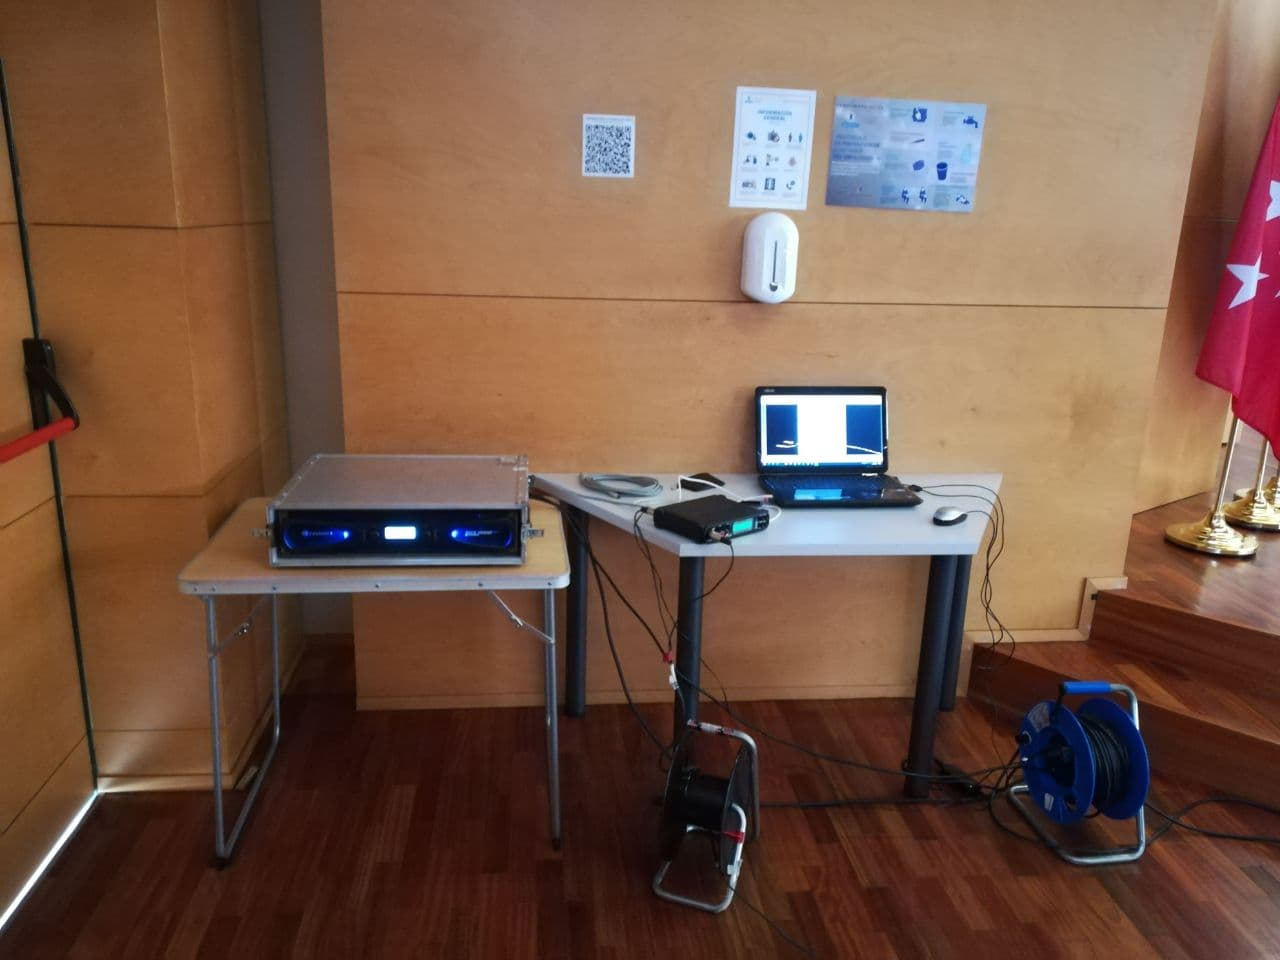
\includegraphics[scale=0.4]{../imagenes/control.jpg}
			    \centering
			    \caption{Disposición de la zona de control para la realización de las grabaciones.}
			    \label{fig:control}
	        \end{figure}
	    
        \subsection{Metodología para la grabación de las respuestas al impulso}
            Una vez escogidas las posiciones de medida y conectados los equipos, se procede a realizar una medida de las condiciones atmosféricas. Más concretamente, se toma una medida de la temperatura y la humedad relativa presente en el recinto. En el día de las medidas se registró una temperatura de 27ºC y una humedad relativa del 34.5\%.
        
            A continuación, se coloca la fuente dodecaédrica en el centro del escenario, que es el punto que se va utilizar para realizar las medidas; también se colocan ambos micrófonos en el trípode y se situa en la posición más lejana respecto de la fuente que se va a medir. Una vez situados, se enciende el amplificador, la tarjeta de sonido y el ordenador. Tras comprobar que el ordenador detecta correctamente la tarjeta de sonido, se inicia el programa ``Dirac''. En él, se acceden a los parámetros de configuración de las medidas fijando las entradas y salidas de la tarjeta de sonido correspondientes. También se determina la señal con la que se van a obtener las respuestas al impulso. En nuestro caso, se opta por un barrido sinusoidal de algo más de cinco segundos de duración. Se opta por esta duración porque el tiempo de reverberación aproximado del salón de actos es de algo más de 1.2 segundos. Por este motivo, el barrido debe tener una duración de al menos el doble de duración y esta opción tiene margen suficiente.
        
            Una vez configurado el software, se realizan varias pruebas de la medida ajustando la ganancia del amplificador de forma que se obtiene una relación señal a ruido suficiente. Para el calculo mediante la estimación del tiempo de reverberación T20, se requiere una relación señal a ruido de 35dB en todas las bandas de frecuencia. Este ajuste se realiza teniendo especial precaución de que la fuente no empiece a distorsionar. Una vez ajustado el amplificador, se repite la medición con los micrófonos situados en la posición más cercana a la fuente para comprobar que los niveles recibidos no saturan.
        
            Con estas comprobaciones realizadas, se procede a la obtención de las respuestas impulsivas. Se comienza desde las filas más alejadas a la fuente y se va avanzando una fila cada vez que se concluye la anterior siguiendo los esquemas presentandos en el apartado de ``Numeración y selección de las posiciones de toma de datos''. Para cada posición, una vez concluidos los dos barridos que realiza el software, se comprueba que la relación señal a ruido en todas las bandas sea superior a 35dB, como se explicó anteriormente. Si se produce algún evento extraño durante la reproducción o se sospecha que la respuesta es errónea, se repite la medición. Este procedimiento se repite en todas las posiciones a lo largo de las dos sesiones de medidas.
        
            Es importante remarcar que se aseguró de que los cables utilizados y la ganancia aplicada es la misma en ambas sesiones. También se repitieron medidas en algunas filas con el fin de comprobar posteriormente que las respuestas son indistinguibles por parte de los oyentes.
        
            Al  final del proceso de toma de datos, se obtuvieron un total de 100 archivos de audio en formato ``.wav'' con la respuesta al impulso obtenida en cada una de las posiciones.
            
            \section{Procesado de los datos - Auralizaciones}
                Una vez obtenidos los datos, se planteó la cuestión sobre qué tipo de audio sería más conveniente: si las respuestas al impulso o bien dichas respuestas convolucionadas con otros audios anecoicos (también conocido como audios auralizados). Para el caso de este proyecto, se ha optado por la segunda opción por varios motivos.
        
                El primero es que las personas están más acostumbradas a escuchar, y por tanto comparar, sonidos de carácter más melódico que se alejan de las respuestas al impulso, las cuales son parecidas al producido por un disparo.
        
                Otro motivo es que este sistema permite escoger un tipo de sonido que se ajuste en buena medida al tipo de evento para los que la sala está pensada con la ventaja añadida de que no se necesita que dicho evento se realice en el momento de las grabaciones.
        
                El audio utilizado está obtenido de la página web de OpenAir de la universidad de York que incluye numerosos audios anecóicos de diferentes cateogrías y también respuestas impulsivas de diferente tipos de espacios grabados por todo el mundo. Particularmente, se escoge la grabación de una voz femenina haciendo una escala musical. Esto se corresponde con el uso principal del Salón de actos que consiste en conferencias y música de coro.
        
                Para la auralización se utiliza el software de Cycling74 ``MaxMSP'' junto con el plugin de la Universidad de Huddersfield, ``\textit{HISSTOOLS}''. Este software permite realizar la convolución de la respuesta al impulso grabada con el audio anecoico de forma que se obtiene el audio auralizado que se desea. Para ello, se crea un pequeño script o ``\textit{patch}'' que realiza dicho procedimiento para todas las respuestas impulsivas previamente grabadas y se almacenan las convoluciones en una nueva carpeta de forma automática. Dicho \textit{patch} puede observarse en la siguiente figura \ref{fig:convolver_max}. Del mismo modo, se incluye una versión texto de dicho script en el Anexo XX.
                
                Por comodidad, se mantiene la misma numeración y terminología para los audios convolucionados que se había seguido para las grabaciones. Siendo la única diferencia la carpeta donde se almacenan.
        
                \begin{figure}[H]
	                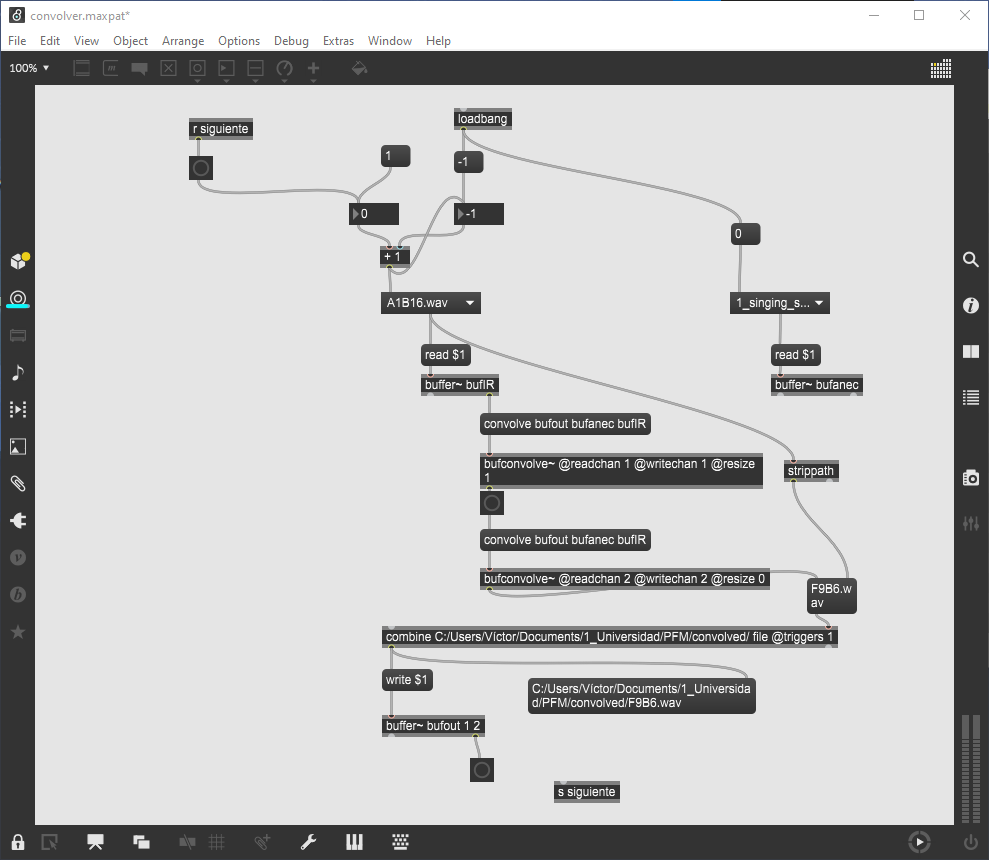
\includegraphics[scale=0.4]{../imagenes/convolver_max.png}
			        \centering
			        \caption{Patch en MaxMSP para la convolución de las respuestas impulsivas con el audio anecoico.}
			        \label{fig:convolver_max}
	            \end{figure}
        
                \newpage
            
    \section{Segunda toma de datos}
        Durante fases posteriores del proyecto, se localizó un error en el procesado de las señales que las hicieron inservibles para el propósito de nuestro proyecto. Debido a esto, y a la adquisición de unos micrófonos biaurales, se decidió realizar una nueva toma de datos con las que realizar el test subjetivo final.
        
        
       \subsection{Numeración y selección de las butacas en la segunda toma de datos}
            Para la segunda toma de datos, se siguió la misma numeración que la vez anterior. Es decir, para las butacas normales, se sigue la estructura ``FxBy'' siendo ``x'' e ``y'' el número de fila y de butaca respectivamente tal y como ya se mostró en el apartado de la primera toma de datos.
                
            Del mismo modo, para las tres filas más próximas al escenario, la numeración utilizada es de la forma ``AxBy'' en la que, de nuevo, ``x'' e ``y'' tienen el mismo significado.\newline
                
            La selección de las posiciones de grabación también sigue el mismo criterio aplicado la otra vez: se selecciona una de cada tres butacas de la mitad derecha del escenario. En la fila siguiente se desplaza la primera butaca una posición a la derecha. Puede volverse a consultar la figura \ref{fig:butacasMarcadas} para observar todas las posiciones de grabación.
                
            Al contrario que la otra vez, esta vez no se han seleccionado las posiciones extremas del lado izquierdo ya que, tras el experimento previo, se vio que los participantes podrían distinguirlos perfectamente. Del mismo modo, como la toma de datos se realizó en un único día, no se repitieron medidas en ninguna posición, aunque tampoco sería necesario porque ya se observó tras el primer test que los oyentes eran incapaces de distinguirlos entre sí.
                
                
        \subsection{Equipo utilizado para la segunda toma de datos}
            Para esta nueva toma de datos, la principal diferencia en torno al equipo utilizado se encuentra en los micrófonos utilizados. En este caso, se utilizaron unos micrófonos biaurales ``Roland CS-10EM''. Estos micrófonos tienen la particularidad de que tienen la forma de auriculares \textit{in-ear} y se conectan mediante un conector mini-jack estéreo. Estos micrófonos necesitan que se les suministe una alimentación de entre 2 y 5 Voltios, algo que no es posible en la tarjeta de sonido MOTU que se utilizó en la anterior toma de datos. Por este motivo, se realiza la grabación de las señales a través de una grabadora de audio externa que permite aplicar dicha alimentación. Para nuestro caso, se ha optado por una ``Yamaha pr7''. En la figura \ref{fig:microsBi} pueden observarse tanto los micrófonos como la grabadora.
                
            \begin{figure}[H]
                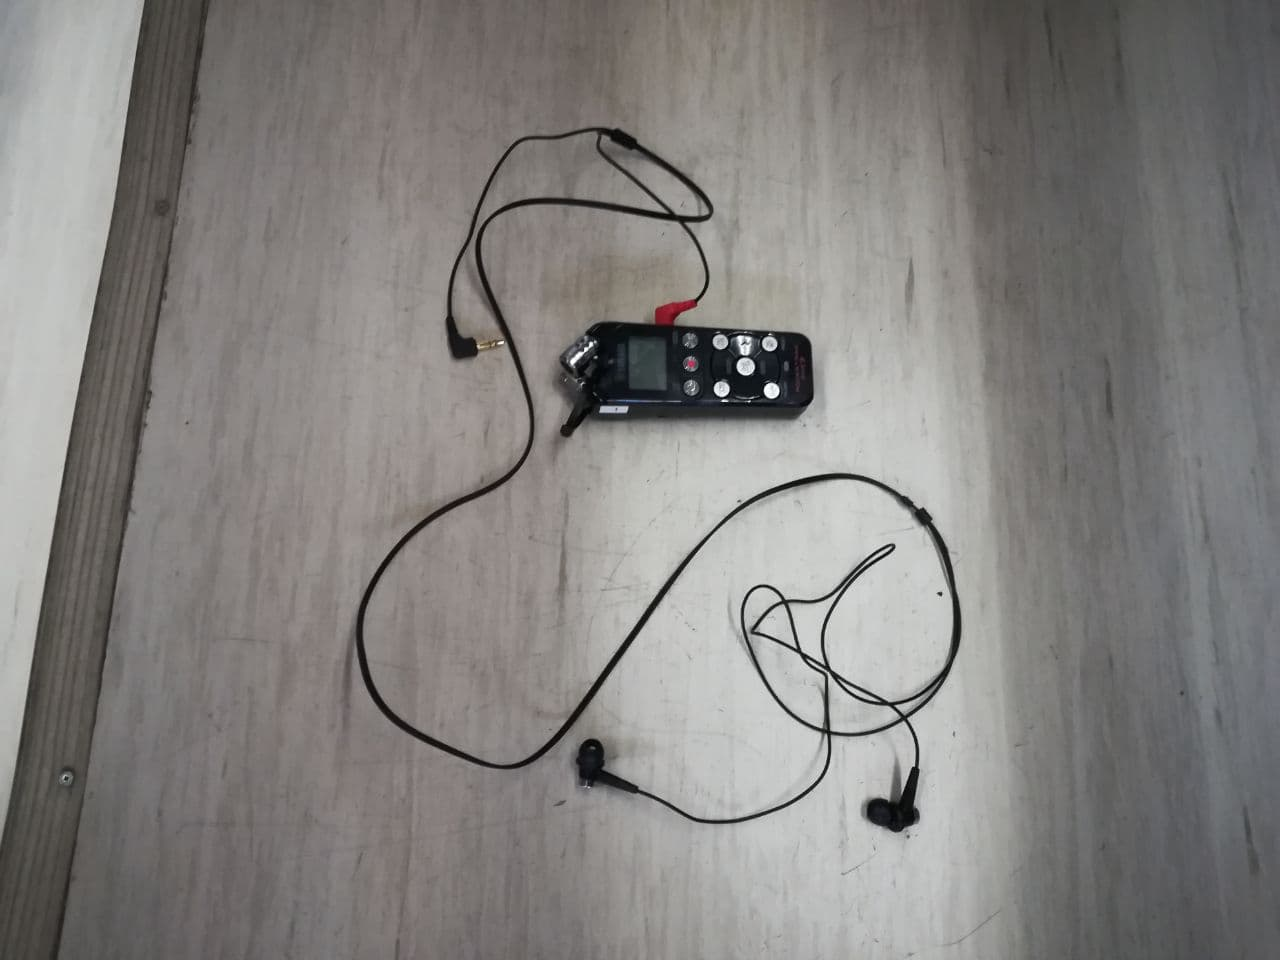
\includegraphics[scale=0.3]{../imagenes/MicroBi.jpg}
                \centering
                \caption{Micrófonos biaurales Roland y grabadora Yamaha utilizada para la grabación de las respuestas.}
                \label{fig:microsBi}
            \end{figure}
                
            La tarjeta de sonido se sigue utilizando para controlar la fuente de sonido dodecaédrica al igual que la vez anterior.
                
            A modo de resumen, se adjunta una nueva lista con todo el equipamiento utilizado para la grabación de las respuestas:
                
            \begin{itemize}
                \item Ordenador portátil ASUS 2 con Windows 10 y software Dirac instalado.
	            \item Tarjeta de sonido MOTU UltraLite-mk3 Hybrid.
	            \item Amplificador de potencia Crown XLS 2002.
	            \item Fuente dodecaédrica.
	            \item Alargaderas y cableado necesario para el conexionado de los equipos.
	            \item Micrófonos biaurales Roland CS-10EM.
	            \item Grabadora portátil Yamaha pr7.
            \end{itemize}
                
            En la figura \ref{fig:equipos}, ya presentada anteriormente, pueden observarse algunas imágenes de algunos de los equipos ya mencionados.
                
        \subsection{Metodología para la grabación de las respuestas al impulso}
            La metodología seguida para la grabación de esta tanda de señales es muy similar a la ya comentada anteriormente.
                
            En primer lugar, se procede a hacer una escucha de las fuentes de ruido que se aprecian dentro del espacio. De esta forma, se localizó un ruido eléctrico debido a la iluminación del salón de actos. Este ruido desaparecía al apagar las luces, por lo que se optó por dejarlas apagadas durante las grabaciones, ya que desde los ventanales entraba luz suficiente para poder realizar el trabajo. Del mismo modo, se localizó un ruido esporádico procedente de uno de los altavoces montados en el escenario. A primera vista parecía debido a algún problema de contacto, pero no había forma de asegurarse. Por suerte, era de un nivel aceptable y su duración era muy escasa de forma que no se percibía mientras se reproducían los barridos.
                
            Una vez analizadas las diferentes fuentes de ruido, se procede a calibrar el sistema de forma que la relación señal a ruido en las posiciones más lejanas respecto de la fuente sean aceptables (mayor o igual a 35dB) y que ni la fuente ni los micrófonos saturaran en ningún momento.
                
            Una vez hecha esta comprobación, se comenzó con las grabaciones. El orden seguido fue desde las filas más alejadas a la fuente a las más cercanas. La persona encargada de ser sujeto de las medidas se colocaba los auriculares y se sentaba en la butaca que correspondía como se aprecia en la figura \ref{fig:Nico}. Una vez colocado, se comenzaba la reproducción de cuatro rondas de barridos frecuenciales de 20Hz a 20kHz. El sujeto debía iniciar manualmente la grabación una vez terminaba de reproducirse el primer barrido y finalizarla una vez terminaba el tercer barrido. Una vez realizada la grabación, se comprobaba que se había grabado correctamente y se pasaba a la siguiente posición. 
                
            \begin{figure}
                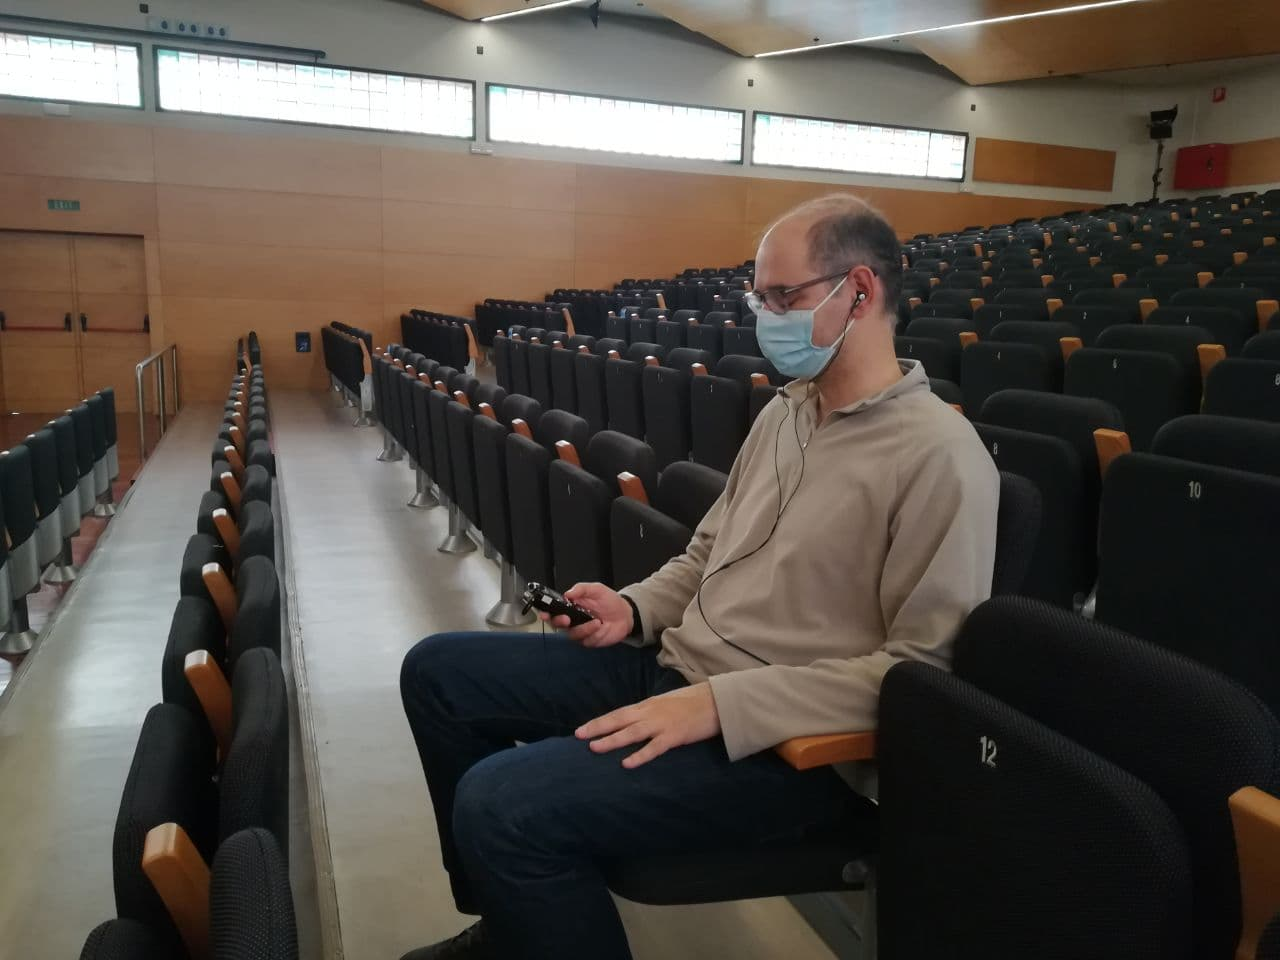
\includegraphics[scale=0.3]{../imagenes/Nico.jpg}
                \centering
                \caption{Ejemplo de la disposición del sujeto para la grabación de las señales.}
                \label{fig:Nico}
            \end{figure}
                
            En total se obtuvieron unas 83 grabaciones que, a continuación, se procesaban en el mismo ordenador utilizando el software Dirac con el fin de obtener las respuestas al impulso. Para ello, se utiliza el mismo menú utilizado en la primera toma de datos, pero esta vez, en vez de realizar una grabación, se importa la señal ya grabada y se le pide al programa que calcule la respuesta al impulso utilizando como señal de referencia la misma utilizada en la reproducción de la fuente. De forma que el programa genera al final un archivo como el que se observa en la figura X.
            
        \subsection{Procesado de los datos}
            Para esta seguna toma de datos, se ha decidido no realizar el proceso de auralización de las señales con los audios anecoicos. Esto se debe a que el proceso de auralización no es perfecto y que, al final, a pesar de que son señales más ``habituales'' para los participantes, no nos aportan nada que no se pueda conseguir reproduciendo diréctamente las respuestas al impulso.
            
            A nivel de procesado para esta parte, sólo se ha recortado la duración del fichero de audio para ajustarlo a la duración de la señal y no hacer que los oyentes escucharan largos tramos de silencio. En ningún momento se modifican las ganancias de las señales para evitar que la información acústica pueda quedar modificada respecto de los valores de grabación. El ajuste de volumen para que sea cómodo se realizará en el test mediante los ajustes de volumen del sistema operativo.
            
    \section{Medida de distancias clave}
        Para un correcto análisis de los resultados, es necesario realizar una serie de medidas en el auditorio. Esto nos permite, más adelante, poder organizar los resultados en función de diferentes referencias y ver si existe alguna relación entre ellas. En nuestro caso, hemos considerado como importantes las distancias de la fuente dodecaédrica a la primera butaca, la distancia entre filas, entre butacas, el ancho del pasillo, entre otras. Todas estas distancias pueden observarse en la figura \ref{fig:distancias}.
        
        \begin{figure}
                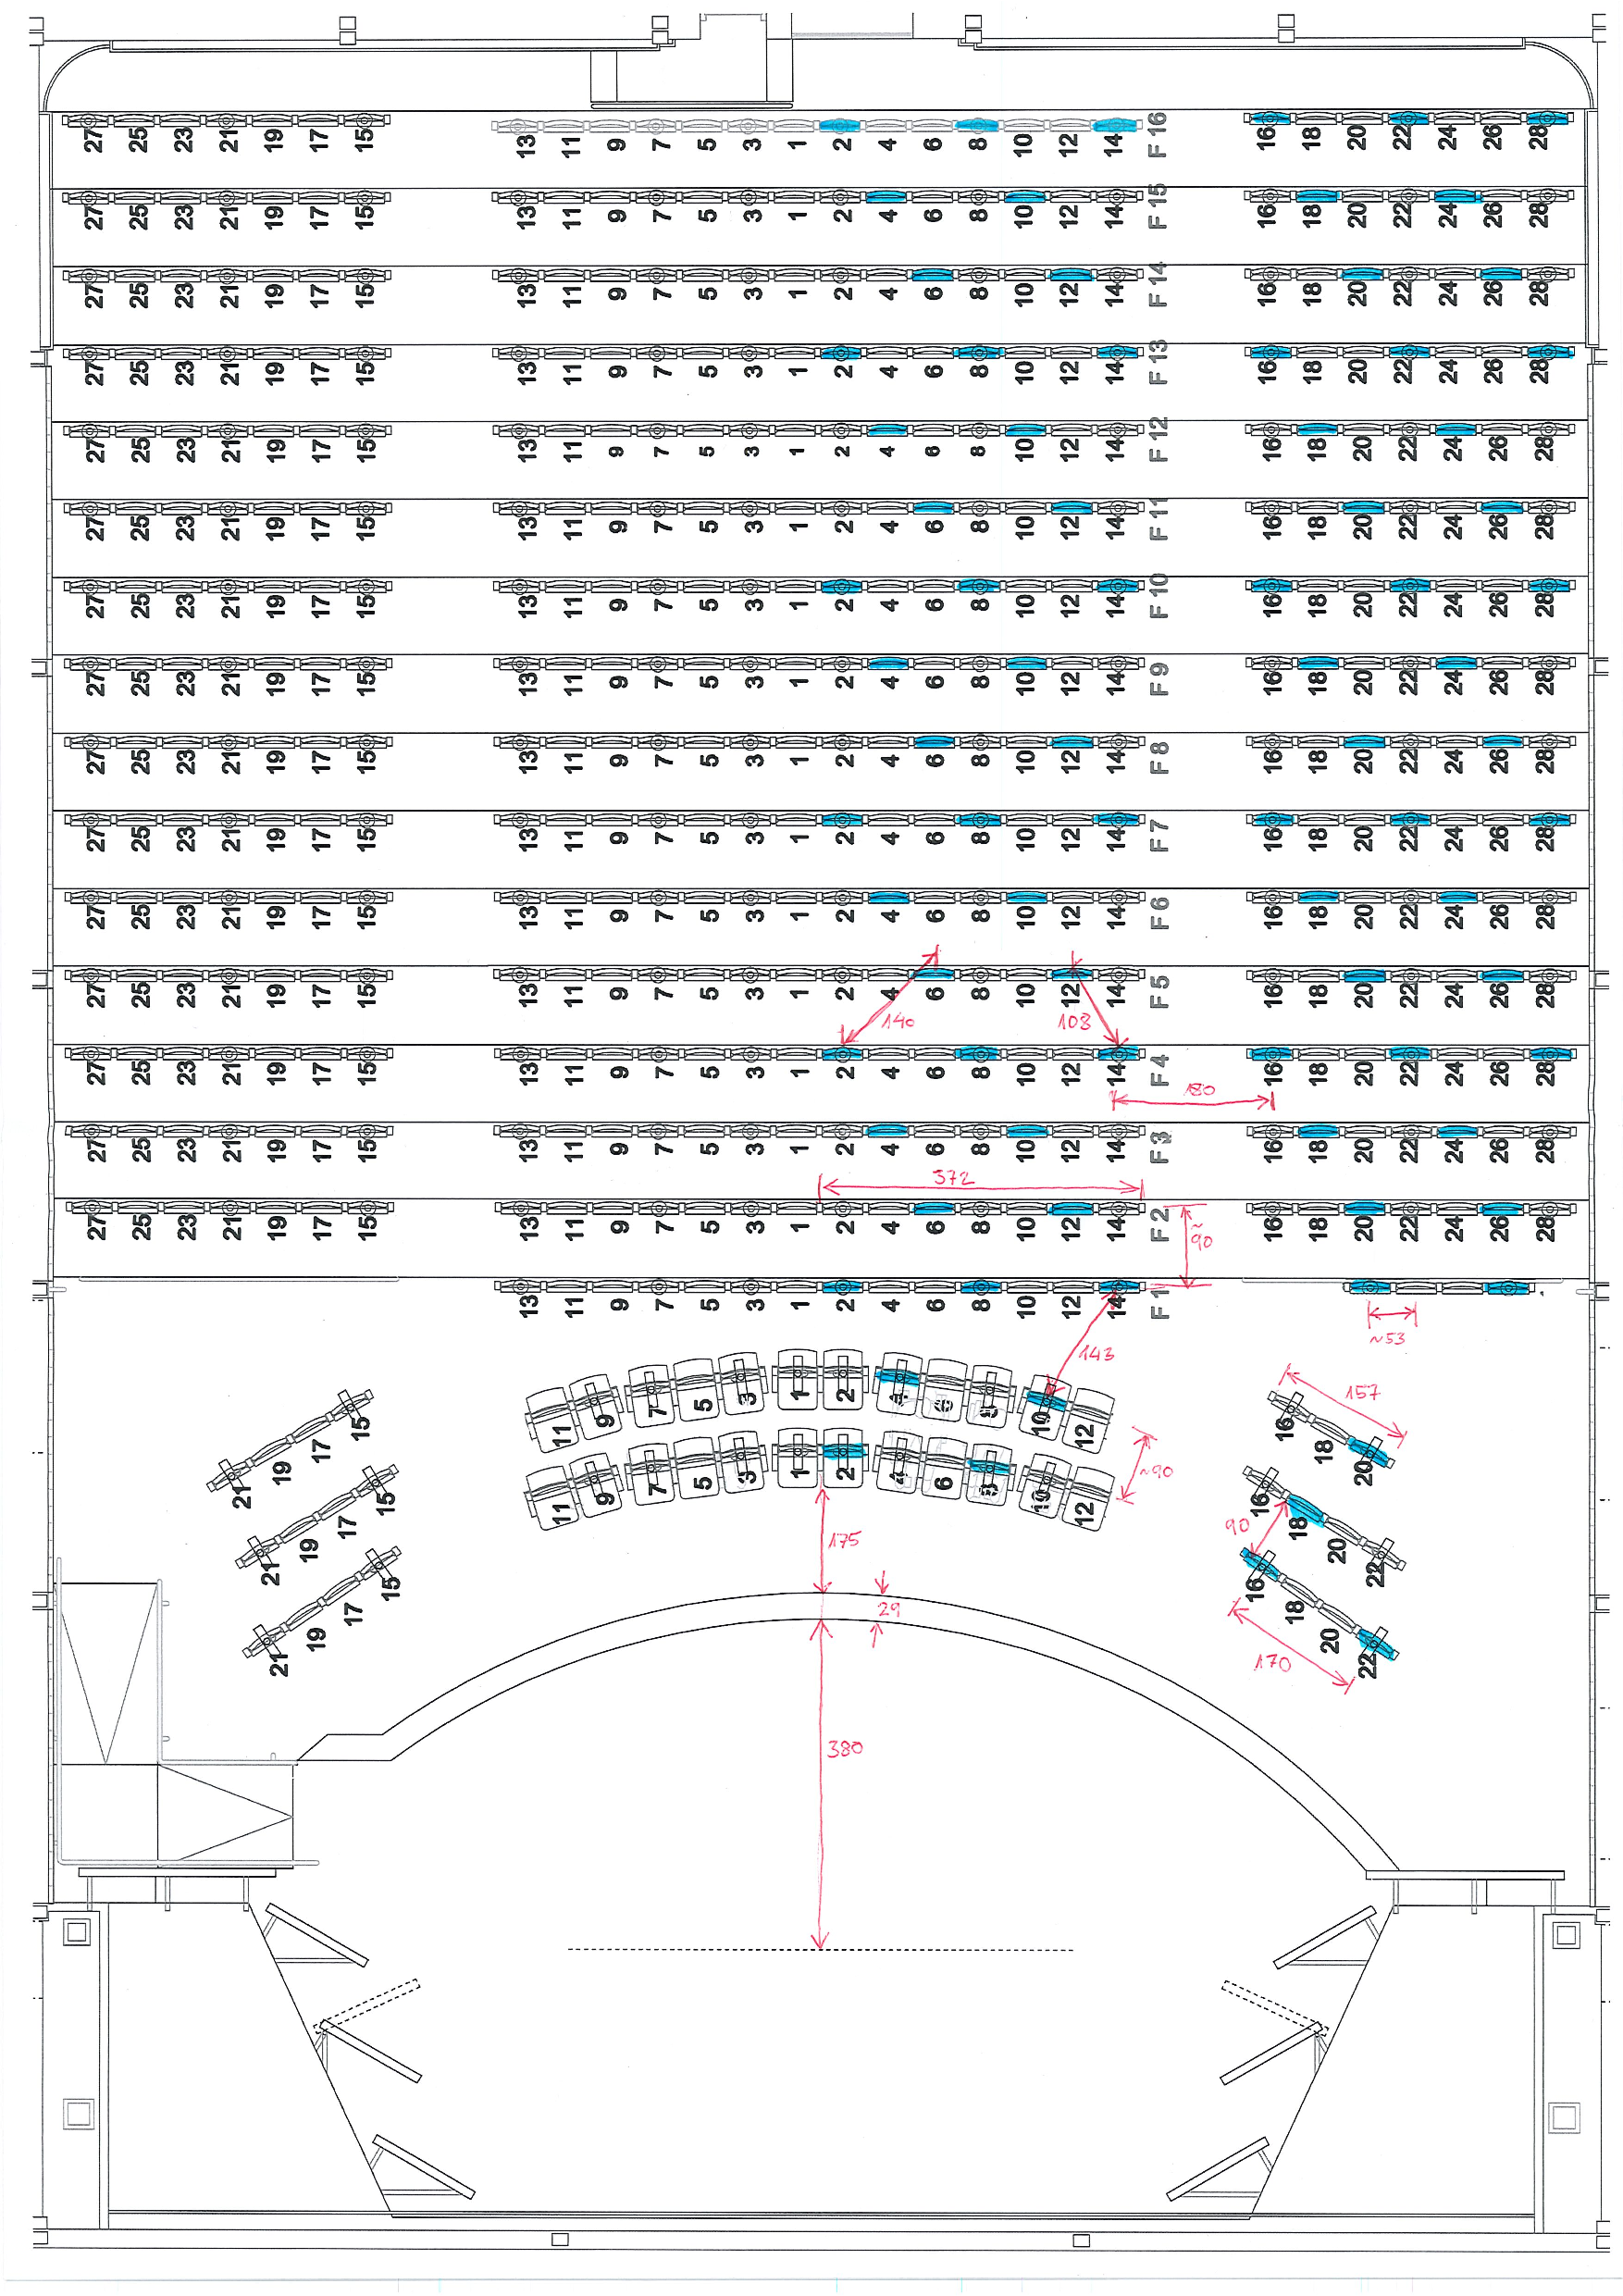
\includegraphics[scale=0.5]{../imagenes/AuditorioMedidasButacas.pdf}
                \centering
                \caption{Medidas de distancias tomadas dentro del auditorio.}
                \label{fig:distancias}
            \end{figure}
        
    

\end{document}